\documentclass[10pt,dvipsnames,enabledeprecatedfontcommands]{scrartcl}
\usepackage{lmodern}
\usepackage{amssymb,amsmath}
\usepackage{ifxetex,ifluatex}
\usepackage{fixltx2e} % provides \textsubscript
\ifnum 0\ifxetex 1\fi\ifluatex 1\fi=0 % if pdftex
  \usepackage[T1]{fontenc}
  \usepackage[utf8]{inputenc}
\else % if luatex or xelatex
  \ifxetex
    \usepackage{mathspec}
  \else
    \usepackage{fontspec}
  \fi
  \defaultfontfeatures{Ligatures=TeX,Scale=MatchLowercase}
\fi
% use upquote if available, for straight quotes in verbatim environments
\IfFileExists{upquote.sty}{\usepackage{upquote}}{}
% use microtype if available
\IfFileExists{microtype.sty}{%
\usepackage[]{microtype}
\UseMicrotypeSet[protrusion]{basicmath} % disable protrusion for tt fonts
}{}
\PassOptionsToPackage{hyphens}{url} % url is loaded by hyperref
\usepackage[unicode=true]{hyperref}
\PassOptionsToPackage{usenames,dvipsnames}{color} % color is loaded by hyperref
\hypersetup{
            pdftitle={Boosting Legal Probabilism},
            pdfauthor={Marcello Di Bello and Rafal Urbaniak},
            colorlinks=true,
            linkcolor=Maroon,
            citecolor=Blue,
            urlcolor=blue,
            breaklinks=true}
\urlstyle{same}  % don't use monospace font for urls
\usepackage{graphicx,grffile}
\makeatletter
\def\maxwidth{\ifdim\Gin@nat@width>\linewidth\linewidth\else\Gin@nat@width\fi}
\def\maxheight{\ifdim\Gin@nat@height>\textheight\textheight\else\Gin@nat@height\fi}
\makeatother
% Scale images if necessary, so that they will not overflow the page
% margins by default, and it is still possible to overwrite the defaults
% using explicit options in \includegraphics[width, height, ...]{}
\setkeys{Gin}{width=\maxwidth,height=\maxheight,keepaspectratio}
\IfFileExists{parskip.sty}{%
\usepackage{parskip}
}{% else
\setlength{\parindent}{0pt}
\setlength{\parskip}{6pt plus 2pt minus 1pt}
}
\setlength{\emergencystretch}{3em}  % prevent overfull lines
\providecommand{\tightlist}{%
  \setlength{\itemsep}{0pt}\setlength{\parskip}{0pt}}
\setcounter{secnumdepth}{5}
% Redefines (sub)paragraphs to behave more like sections
\ifx\paragraph\undefined\else
\let\oldparagraph\paragraph
\renewcommand{\paragraph}[1]{\oldparagraph{#1}\mbox{}}
\fi
\ifx\subparagraph\undefined\else
\let\oldsubparagraph\subparagraph
\renewcommand{\subparagraph}[1]{\oldsubparagraph{#1}\mbox{}}
\fi

% set default figure placement to htbp
\makeatletter
\def\fps@figure{htbp}
\makeatother

%\documentclass{article}

% %packages
 \usepackage{booktabs}
 \usepackage[sort&compress]{natbib}
\usepackage{graphicx}
\usepackage{longtable}
\usepackage{ragged2e}
\usepackage{etex}
%\usepackage{yfonts}
\usepackage{marvosym}
\usepackage[notextcomp]{kpfonts}
\usepackage{nicefrac}
\newcommand*{\QED}{\hfill \footnotesize {\sc Q.e.d.}}
\usepackage{multicol} 
%\usepackage[textsize=footnotesize]{todonotes}
%\linespread{1.5}

\usepackage{xcolor}

\setlength{\parindent}{10pt}
\setlength{\parskip}{1pt}


%language
%\usepackage{times}
\usepackage{mathptmx}
\usepackage[scaled=0.88]{helvet}

\usepackage{t1enc}
%\usepackage[utf8x]{inputenc}
%\usepackage[polish]{babel}
%\usepackage{polski}

\usepackage{subcaption}


%AMS
\usepackage{amsfonts}
\usepackage{amssymb}
\usepackage{amsthm}
\usepackage{amsmath}

%\usepackage{geometry}
 %\geometry{a4paper,left=35mm,top=20mm,}

%abbreviations
\newcommand{\ra}{\rangle}
\newcommand{\la}{\langle}
\newcommand{\n}{\neg}
\newcommand{\et}{\wedge}
\newcommand{\jt}{\rightarrow}
\newcommand{\ko}[1]{\forall  #1\,}
\newcommand{\ro}{\leftrightarrow}
\newcommand{\exi}[1]{\exists\, {_{#1}}}
\newcommand{\pr}{\mathsf{P}}
\newcommand{\odds}{\mathsf{Odds}}
\newcommand{\ind}{\mathsf{Ind}}
\newcommand{\nf}[2]{\nicefrac{#1\,}{#2}}
\newcommand{\R}[1]{\texttt{#1}}

\newtheorem{q}{\color{blue}Question}


%% Rafal's stuff
\usepackage[margin=1.5in,top=1in]{geometry}
\usepackage[textsize=scriptsize, textwidth = 3cm]{todonotes}
% This is my own comment shading, keep \todo for general stuff, feel free to define your own separate comment colors (usually useful if you use margin comments at tall) For instance, I defined one for Patrycja
\newcommand{\rt}[1]{\todo[color = orange!40]{#1}}
\newcommand{\pt}[1]{\todo[color = blue!40]{#1}}




\newtheorem*{reply*}{Reply}
\usepackage{enumitem}
\newcommand{\question}[1]{\begin{enumerate}[resume,leftmargin=0cm,labelsep=0cm,align=left]
\item #1
\end{enumerate}}

\usepackage{float}

% \setbeamertemplate{blocks}[rounded][shadow=true]
% \setbeamertemplate{itemize items}[ball]
% \AtBeginPart{}
% \AtBeginSection{}
% \AtBeginSubsection{}
% \AtBeginSubsubsection{}
% \setlength{\emergencystretch}{0em}
% \setlength{\parskip}{0pt}

\title{Boosting Legal Probabilism}
\author{Marcello Di Bello and Rafal Urbaniak}
\date{}

\begin{document}
\maketitle

\section{The Book}\label{the-book}

\subsection{Brief Description}\label{brief-description}

\footnotesize In one or two paragraphs, describe the work, including its
rationale, approach, and pedagogy. (This book is\ldots{} It does\ldots{}
Its distinguishing features are\ldots{})

\normalsize

Can the evidence presented at trial be examined, weighed and assessed
using probability theory? Can legal decision-making and standards of
proof such as `preponderance of the evidence' or `proof beyond a
reasonable doubt' be defined using the language of probability? Does the
deployment of probability theory in assessing evidence and making
decisions improve the accuracy and fairness of legal decision-making?
Over the last fifty years, these questions have been debated in the
literature in philosophy, law, forensic science and artificial
intelligence. Legal probabilism is a research program whose supporters
believe the answer to these questions is, by and large, affirmative.
Others, however, hold a less optimistic view. `Boosting Legal
Probabilism' examines the most important objections to this research
program and articulates a version of legal probabilism that is able to
address many, if not all, of these objections.

We begin with the simple version of the theory. It comprises two key
elements: first, Bayes' theorem for assessing the weight of the
evidence, and second, probability thresholds as decision criteria. The
simple version of legal probabilism has much to be reccomeded for, but
also falls prey to several difficulties, including the problem of
conjunction, puzzles of naked statistical evidence, the problem of
priors. Some legal probabilists have attempted to dismiss these
difficulties or downplay their significance. We confront them at face
value and show that they cannot be addressed within the confines of
simple legal probabilism. We then develop a more sophisticated theory,
what we call legal probabilism 1.02, which takes advatange of Bayesian
networks and other seminal ideas in the literature in forensic science
and artificial intelligence. `Boosting Legal Probabilism' articulates
the first comprehensive philosophical analysis of whether---and if so,
to what extent---legal probabilism 1.02 can overcome the limitations of
simple legal probabilism. We show that the more sophisticated version
significantly improves on the simple version and rivals in explanatory
power two competing accounts of judicial fact-finding: argumentation
theory and relative plausibility. To add precision to the claims made in
the book, the analytical argument is supplemented with an
\textbf{\textsf{R}} code implementation.

`Boosting Legal Probabilism' is aimed at philosophers with an interest
in legal epistemology and epistemology more generally. Many of the
difficulties of legal probabilism resemble difficulties faced by
Bayesianism in epistemology. The book will also draw attention outside
philosophy from legal scholars who have championed applications of
probability theory to evidence law as well as scholars who have resisted
this trend. Another target audience includes computer scientists and
psychologists interested in studying evidential reasoning and
decision-making under uncertainty. Besides contributing to the
literature about legal probabilism, the book aims to introduce
unfamiliar readers to the rich interdisciplinary debate on the topic,
often scattered throughout journals and books in philosophy, law,
computer science, forensic science and psychology. So the book is aimed
at scholars, advanced undergraduates and curios readers more generally.
Some chapters present original research and require technical background
in probability theory. Others are introductory, suitable for an advanced
undergraduate course.

\subsection{Outline}\label{outline}

\noindent
\textbf{Part I - Legal Probabilism and Its Foes}

\noindent
The first part of the book will instill interest in legal probabilism
among unfamiliar readers and refresh seasoned readers about the main
points of contention. \textbf{Chapter 1} outlines simple legal
probabilism which comprises a familiar repertoire: Bayes' theorem,
likelihood ratios, probability thresholds, expected utility
maximization. This repertoire has proven useful in several ways,
especially in the assessment of explicitly quantitative evidence such as
DNA matches and other expert evidence. At the same time, as
\textbf{Chapter 2} shows, simple legal probabilism is liable to a host
of conceptual difficulties: the conjunction problem, the problem of
priors, paradoxes of naked statistical evidence. These difficulties are
well-known. Others are less familiar: the problem of complexity, soft
variables, the difficulty with corroboration.

The first two chapters provide the essential background for a deeper
examination of legal probabilism and the development of its more
sophisticated version. The remaining parts of the book cover two
distinct topics: evidence assessment (Part II and Part III, Chapters 3
through 10) and decision-making (Part IV and Part V, Chapters 11 through
17). This distinction reflects the fact that legal probabilism is both a
theory of evidence assessment (or evidence evaluation, evidence
weighing) as well as a theory of decision-making at trial. These two
topics are obviously intertwined in important ways, but are best kept
separate for analytical clarity.

\vspace{3mm} \noindent
\textbf{Part II - Evidence Assessment First Pass}

\noindent
The second part of the book discusses in great detail two formal tools
that are essential for the legal probabilist: Bayes' theorem and
likelihood ratios. We focus in particular on how these tools can help to
assess, weigh and evaluate evidence at trial as well as what their
limitations are.

\textbf{Chapter 3} begins with Bayes' theorem and surveys many of its
applications, for example, as a tool to avoid reasoning fallacies such
as the prosecutor's fallacy and the base rate fallacy. At the same time,
its applications are also limited. As discussed in \textbf{Chapter 4},
court cases often require fact-finders to weigh several pieces of
evidence, sometimes conficting and susceptible to different
interpretations. The hypotheses that the fact-finders are asked to
evaluate in light of the evidence are structured stories or explanations
constituted by several sub-propositions. This level of complexity can
hardly be modeled by sucessive discrete applications of Bayes' theorem.
A more sophisticated machinery for evidence assessment is needed.

\textbf{Chapter 5} describes a formal tool distinct from Bayes' theorem
which many legal probabilists have found useful: likelihood ratios.
Bayes' theorem requires one to assess the prior probabilities of the
hypothesis of interest. The problem is that assessing prior
probabilities is notoriously difficult. Likelihood ratios, instead,
offer a way to evaluate the evidence presented at trial without the need
of assessing prior probabilities. We illustrate the applications of
likelihood ratios focusing on the debate about cold-hit DNA matches. The
chapter also examines the weaknesses of this approach. The choice of the
competing hypotheses compared in the likelihood ratio is often a source
of confusion, manipulation and subjective judgment. Another problem is
that, like simple applications of Bayes' theorem, likelihood ratios are
still unable to model complex bodies of evidence. A further problem, as
critics have alleged, is that likelihood ratios cannot model the notion
of evidential relevance.

\vspace{3mm} \noindent
\textbf{Part III - Evidence Assessment More and Better}

\noindent
Chapters 3 and 4 show that we need to move past simple legal
probabilism. Chapter 5 shows that likelihood ratios, while useful in
many ways, are still an unsatisfactory approach overall. The journey
toward legal probabilism 1.02 is accomplished in Part III, Chapters 6
through 10. Our analysis is informed by the following working
hypothesis. An accusation of liability must be substantiated by
providing a well-specified account -- a story or narrative -- of the
alleged illegal act committed by the defendant. This account consists of
several moving parts, each supported by different items of evidence. The
defense may respond by attacking the supporting evidence, the internal
consistency of the account, or by offerring an alternative account. It
is this complex dynamics that we aim to formalize in the following
chapters.

We focus on two aspects of the evaluation of trial evidence which simple
legal probabilism is unable to model: first, judges and jurors often
think holistically about the evidence, say in terms of coherent stories
or explanations, without assessing the evidence by discrete applications
of Bayes' theorem or likelihood ratios; second, different pieces of
evidence interact in complex relationships, such as undercutting,
rebutting, converging, corroborating evidence. We show that Bayesian
networks constitute the formal machinery necessary for developing a more
sophisticated legal probabilism that is able to capture these phenomena.
The key idea is that the coherence of a story as well as conflicts
between pieces of evidence can be modeled formally by corresponding
properties of, operations on, and relations between Bayesian networks.

\textbf{Chapter 6} offers a crash course on Bayesian networks with a
focus on the assessment of legal evidence. A Bayesian network comprises
a directed acyclic graph (called a DAG) that represents relations of
dependence between variables, along with conditional probability tables
corresponding to these relations. In the last decade, the literature in
artificial intelligence and forensic science has made significant
progress in modeling holistic notions such as the coherence of a story
and argument-based notions such as conflicts between pieces of evidence.
Chapter 6 surveys this literature focusing on the work of Charlotte Vlek
and Norman Fenton. Vlek, together with Bart Verheij and Henry Prakken,
proposed to model the coherence of a story by adding a node in the
Bayesian network, call it a `story node'. The story node has other nodes
as its children corresponding to the events that make up the story. In
turn, these events are linked to their supporting evidence. An example
of a Bayesian network with a story node (or scenario node to use Vlek's
terminology) is depicted below:

\begin{center}
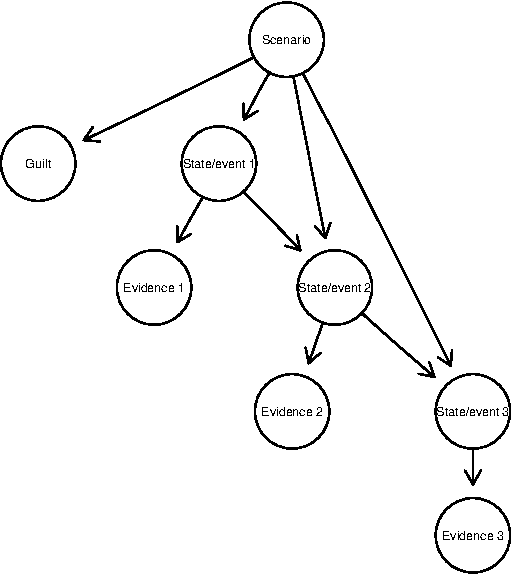
\includegraphics[width=8cm]{vlek-scenario-node.pdf}
 \end{center}

Since the story node unifies the different parts of a story, changes in
the probabilities of these parts can be used to model the notion of
coherence. The stronger the (positive) probabilistic dependence between
the different parts, the more coherent the story. To model conflicts of
evidence, a Bayesian network can be built that comprises two competing
stories, say, one story was put forward by the prosecution and another
by the defense, each supported by their own evidence. The network would
specify that these stories are incompatible and cannot be true
concurrently. Another approach to model conflicting evidence and
competing stories was developed by Norman Fenton and his research group.
Separate stories are represented by separate Bayesian networks, and
Bayesian model comparison is then used for assessing the comparative
evidential support of the competing stories.

\textbf{Chapter 7} focuses on Vlek's story node approach as an account
of coherence. The chapter contains a critical argument followed by a
positive proposal. We show that adding a story node by fiat -- without
any good reason for supposing that the different parts of the story are
connected other than being part of one story -- introduces unnecessary
probabilistic dependencies between the elements of a story. In addition,
the story node approach is overly simplistic as an account of coherence
and fails to engage with the rich philosophical literature on the topic.
After the critical argument, the chapter articulates a more adequate
probabilistic account of coherence. Instead of adding a story node, we
show that it is more appropriate to assess the dependence between the
different parts of a story on a case-by-case basis and build the
Bayesian network accordingly. We then define a formal notion of `story
coherence' that reflects properties of the Bayesian network used to
model the evidence. We show that our formal notion of coherence
addresses the objections against probabilistic accounts of coherence in
the philosophical literature.
\todo{M: ANYTHING ELSE TO DESCRIBE THE POSITIVE ACCOUNT?}

\textbf{Chapter 8} focuses on conflicts between pieces of evidence.
Neither Vlek's story node approch nor Fenton's model comparison approach
adequately capture how pieces of evidence and competing stories may
conflict with one another. It is too simplistic to posit that the
complex adversarial dialectic that takes place in a trial could be
modeled by averaging different Bayesian networks (Fenton) or postulating
relationships of incompatibility between different story nodes (Vlek).
We need an account of more fine-grained notions, such as undercutting
and rebutting evidence, and more generally we need an accounf of how
cross-examimation operates at trial. What cross-examination often
accomplishes is not so much the creation of an alternative story, but
rather, the reinterpretation of an existing story by supplying
additional information. We show that this process of reintepretation can
be represented formally as the refinement of an existing Bayesian
network. Conflicts between pieces of evidence such as undercutting and
rebutting can be modeled by drawing additional arrows between evidence
nodes and hypothesis nodes.

The reverse of the phenomenon of conflicting evidence is that of
converging evidence, in particular, the fact that one piece of evidence
corroborates another. Corroboration has been the focus of extensive
scholarly debate often independently of the debates within legal
probabilism. \textbf{Chapter 9} surveys the literature on corroboration
and the main difficulties that have been levelled against proposed
probabilistic accounts. The chapter then formalizes a notion of
corroboration using Bayesian networks that overcomes most of the
difficulties of exisisting accounts.
\todo{M: ANYTHING ELSE TO DESCRIBE THE POSITIVE ACCOUNT?}

\textbf{Chapter 10} draws some general morals after comparing legal
probabilism 1.02 -- as fomulated in the previous two chapters -- to
other accounts of judicial fact-finding, in particular, argumentation
theory and relative plausibility. Argumentation theory is well suited to
model conflicts between evidence, but cannot easily model the fact that
evidence may conflict more or less strongly with other evidence. Unlike
argumentation theory, legal probabilism 1.02 offers an account of
evidential support, conflict and convergence that captures how these
relations come in degrees of strength. The other competing theory we
consider, relative plausibility, is often criticized because the defense
lawyer need not present a full-fledged alternative story. Without
settling this controversy, we note that legal probabilism 1.02 is
flexible enough to model competing stories (in agreement with relative
plausibility) or model conflicts without the need to construct a
full-fledged alternative story (as critics of relative plausibility
prefer).

Legal probabilism 1.02 can still be challenged because of its
questionable emprical adequacy since judges and jurors hardly follow
probability theory. Nevertheless, we emphasize how legal probabilism
1.02 offers a richer account of evidential support beyond what critics
have recognized. Susan Haack, for example, criticized legal probabilism
for its monodimensional account of evidential support. This is true of
simple legal probabilism in which evidential support is modeled by the
posterior probability of a hypothesis given the evidence or the
likelihood ratio. Legal probabilism 1.02, however, offers a richer
account. In it, evidential support also depends on the degree of
specificity and coherence of the story put forward, and the extent to
which the supporting evidence withstands objections. These features --
specificity and coherence, as well as resistance to objections -- can
serve to formulate decision criteria that are not unidimensional
thresholds. This point is discussed more extensively in the next part of
the book.

\vspace{3mm} \noindent
\textbf{Part IV - Decision-making}

\noindent
The third part of the book examines trial decision-making, specifically,
to what extent standards of proof such as `preponderance of the
evidence' and `proof beyond a reasonable doubt' can be understood
through the lenses of probability theory. There has been a spur of
research arguing that legal probabilism is unfit to model standards of
proof. But this research often holds a narrow view of legal probabilism.
We show that the version formulated in the previous chapters of the book
provides an adequate framework for theorizing about standards of proof.

\textbf{Chapter 11} examines different strategies for theorizing about
standards of proof using probabilistic language. We begin with the most
natural decision criterion, a probability threhsold whose stringency is
determined by expected utility maximization. This account falls prey to
well-known objections, most notably, the puzzles of naked statistical
evidence and the difficulty with conjunction (discussed in greater
detail in later chapters). We then turn to alternative accounts, in
particular, the comparative strategy (Cheng) and the likelihood ratio
strategy (Dawid, Kaplow, Sullivan). Finally, we present our own
proposal. That is, the standard of proof is a function of several
criteria: the probability of liability, the specificity and coherence of
the accusatory story, the comprehensiveness of the supporting evidence
and its ability to withstand objections. In the following chapters, we
show that our proposal outperforms the comparative strategy and the
likelihood ratio strategy. We emphasize that these criteria --
probability, specificity, etc. -- can be modeled using Bayesian
networks. So our proposal lies within the confines of legal probabilism,
though not the narrow version its critics have in mind.

\textbf{Chapter 12} tackles the puzzles of naked statistical evidence.
This is a topic of enormous scholarly attention in the recent
philosophical literature. Our solution rests on two premises. First, an
accusation of liability should be substantiated by a well-specified
account -- or story, narrative -- whose moving parts are each supported
by adequate evidence. In cases of naked statistical evidence, the
probability of liability is high, but the specificity of the
accompanying narrative is suspiciously low. The second premise is that
the supporting evidence should typically be `causally grounded'. This
grounding contributes to a well-specified story and is achieved during
cross-examination by eliciting additional information about the relation
between the evidence and the alleged facts -- for example, information
about the visibility conditions; the academic credential of an expert
witness; the chain of custody of a document. Interestingly, naked
statistical evidence blocks cross-examination because no undercutting
evidence can in principle be brought against it.

\textbf{Chapter 13} tackles another central problem for legal
probabilism, the difficulty with conjunction. We first provide a
detailed argument for why previous attempts in the literature on legal
probabilism have failed. We focus on the likelihood ratio approach by
Dawid and the comparative strategy by Cheng. Our proposal follows the
holistic approach by Allen and Pardo. As noted already, our working
hypothesis is that the prosecution (or the plainitiffi in a civil trial)
should aim to establish a well-specified accusatory narrative whose
moving parts are supported by adequate evidence. Once the prosecution
has accomplished that -- and its case withstands criticism -- each
element of the accusation is estalished to the required standard if and
only if the conjunction of these elements (that is, the story as a
whole) is estalished to the required standard. So long as legal
probabilism can offer an account of evidenetial support that is
sensitive to holistic notions such as coherence and specificity, as well
as argument-based notions such as resistance to objections, legal
probabilism can address the difficulty with conjunction.
\todo{M: THIS MIGHT NEED SOME WORK. WHAT TO ADD?}

\textbf{Chapter 14} compares our probabilistic account of
decision-making and standards of proof to other accounts in the
literature. We advance two main points of criticism. First, other
accounts are not necessarily incompatible with legal probabilism 1.02
which may in fact provide a more riguours way to express their insights.
This point applies to foundeherentism (Hack), normic support (Smith),
argumentation theory (Sartor and Prakken) and to some extent relative
plausibility (Allen and Pardo). The second criticism we make is that
other accounts are engaged with what we might call `epistemology
fetichism' -- that is, they borrow ideas that are popular in
contemporary analytic epistemology and force them onto legal-decision
making. This criticism applies in particular to knowledge accounts of
legal proof.

\vspace{3mm} \noindent
\textbf{Part V - Accuracy and Fairness}

\noindent
Even if one did not agree that legal probabilism as we have articulated
it is helpful for understanding evidence assessment and decision-making
at trial, it can still play an analytical role in theorizing about trial
decisions The fourth part of the book illustrates this point by
discussing two important legaal values that should inform trial
proceedings: accuracy and fairness.

\textbf{Chapter 15} DESCRIPTION. GENERAL TREATMENT OF WHAT VALUES SHOULD
INFORM AND GUIDE TRIAL DECISIONS, SUCH AS FAIRNESS, ACCURACY,
JUSTIFICATION, PUBLIC ANSWERABILITY, DETERRENCE, RESPECT, HUMANITY, ETC.

\textbf{Chapter 16} examines what it means for trial decisions to be
accurate. Evene though many hold that trial decisions should be
accurate, this claim leaves open what we mean by `that.'accuracy' There
are in fact several distinct ways to understand accuracy in trial
decisions, and probability theory offers a language to formulate them.
Accuracy can be understood, among other things, as predictive accuracy
or diagnostic accuracy. The former is the probability that if the
defedant is found (not) liable at trial, the defendant is actually (not)
liabile; the latter is the probability that if the defendant is (not)
liable, the defendant would (not) be found liable at trial. The two
notions are related but they are not equivalent. Distinguishing them has
implications for how we should understand standards of proof. We argue
that diagnostic accuracy, rather than predictive accuracy, is the most
adequate for trial decisions.

\textbf{Chapter 17} turns to the fairness of trial decisions. Another
notion that can be further clarified through the lenses of probability
theory is fairness. What does it means for trial decisions to be fair?
The formalistic sense of fairness would require that every rules be
applied to all participants in the same way. The more substantive sense
of fairness would require that burdens (and benefits) be evenly
distributed across different defendants. Substantive fairness can be
understood as the requirement that all defendants be exposed to the same
risk of mistaken conviction (or more precisely, that the conditional
probability that a defedant, if innocent, would be convicted be the same
across all defendants). Once this notion of substantive fairness is on
the table, we can meaningfully debate whether certain types of evidence
(and types of rules of procedure) are unfair, or whether, as some have
argued, trial decisions are inevitably unfair because evidence is
distributed unfairly via structural inequalities in society.

\textbf{Chapter 18} draws some conclusions and points to open problems
for legal probabilism. \todo{M: ANYTHING TO ADD HERE?}

\vspace{3mm} \noindent
\textbf{Table of contents}

\renewcommand{\labelenumi}{\Roman{enumi}}
\renewcommand{\labelenumii}{\arabic{enumii}}
\renewcommand{\labelenumiii}{\arabic{enumii}.\arabic{enumiii}}

\begin{enumerate}
\item Legal probabilism 1.01 and its foes
\begin{enumerate}

  \item The emergence of legal probabilism
  \begin{enumerate}
  \item  Famous cases
  \item  Probabilistic evidence
  \item  Trial by mathematics
  \item  Some history
  \end{enumerate}
  

  
  \item  A skeptical perspective
  \begin{enumerate}
  \item  The difficulty about conjunction
  \item  The problem of priors
  \item  Naked statistical evidence
  \item  The complexity problem
  \item  Soft variables
  \item  Corroboration
  \item  The reference class problem
  \item  Non-probabilistic theories
  \end{enumerate}


\end{enumerate}
\item  Evidence assessment First Pass


\begin{enumerate}


\setcounter{enumii}{2}
  \item  Bayes' Theorem and the usual fallacies
  \begin{enumerate}
  \item  Assuming independence
  \item  The prosecutor's fallacy
  \item  Base rate fallacy
  \item  Defense attorney's fallacy
  \item  Uniqueness fallacy
  \item  Case studies
  \end{enumerate}

  
  
  \item  Complications and caveats
  \begin{enumerate}
  \item  Complex hypotheses and complex bodies of evidence
  \item Source, activity and offense level hypotheses
  \item  Where do the numbers come from?
  \item  Modeling corroboration
  \item  Stories, explanations and coherence
  \end{enumerate}

  
  \item  Likelihood Ratios and Relevance
  \begin{enumerate}
  \item Likelihood ratio as a measure of evidence strength
  \item The risk of false positive and its impact
  \item Hypothesis choice
  \item Levels of hypotheses and the two-stain problem
  \item Relevance and the small-town murder scenario
  \item The cold-hit confusion
  \item  Likelihood ratio and  cold-hit DNA matches
  \end{enumerate}


\end{enumerate}
\item  Evidence assessment More and Better
\begin{enumerate}

\setcounter{enumii}{5}
\item  Bayesian Networks

  \begin{enumerate}
  \item  Bayesian networks to the rescue
  \item  Legal evidence idioms
  \item Scenario idioms
  \item Modeling relevance
  \item  Case study: Sally Clark
  \item DNA evidence
  \end{enumerate}
  
   \item Coherence
  \begin{enumerate}
  \item  Existing probabilistic coherence measures
  \item  An array of counterexamples
  \item Coherence of structured narrations with Bayesian networks
  \item  Application to legal cases
  \end{enumerate}
  
  
  \item Conflicts
  \begin{enumerate}
  \item Argumentation theory
  \item Undercutting and rebutting evidence
  \item Cross-examination
  \item Conflicting evidence in Bayesian networks
  \end{enumerate}
 
 
  \item Corroboration
  \begin{enumerate}
  \item Boole's formula and Cohen's challenge
  \item  Modeling substantial rise in case of agreement
  \item Ekel\"of's corroboration measure and evidentiary mechanisms
  \item General approach with multiple false stories and multiple witnesses
  \end{enumerate}


  \item  Towards Legal Probabilism 1.02
    \begin{enumerate}
    \item Outperforming competing accounts
    \item Empirical adequacy
    \item Specificity and coherence
    \item Resistance against objections 
    \item Bayesian network implementation
    \end{enumerate}


\end{enumerate}
\item  Standards of proof
\begin{enumerate}


\setcounter{enumii}{10}
 \item  Are Standards of Proof Threhsolds?
  \begin{enumerate}
  \item  Legal background
  \item  Probabilistic thresholds
  \item  Theoretical challenges
  \item  The comparative strategy
  \item  The likelihood strategy
  \item  Probabilistic thresholds revised
  \item  Bayesian networks and probabilistic standard of proof
  \end{enumerate}


\item  Naked statistical evidence
  \begin{enumerate}
  \item  Forty years of hypotheticals
  \item  Specific narratives
  \item  Cross-examination and causal grounding
  \item  Bayesian networks and naked statistical evidence
  \item  Are cold-hit DNA matches naked statistics?
  \end{enumerate}
  
  
\item  The Difficulty with Conjunction
  \begin{enumerate}
  \item  The problem
  \item  The likelihood strategy
  \item  The comparative stratgey
  \item  The holistic strategy
  \item  Complex bodies of evidence and structured narratives
  \end{enumerate}  

 \item  Other accounts 
  \begin{enumerate}
  \item  Baconian probability
  \item  Sensitivity
  \item  Normic Support
  \item  Foundherentism
  \item  Relevant alternatives
  \item  Knowledge
  \item  Relative Plausibility
  \item  Arguments
  \end{enumerate}

\end{enumerate}
\item  Accuracy and Fairness
\begin{enumerate}

\setcounter{enumii}{14}
  \item  The functions of the proof standards
  \begin{enumerate}
  \item  Conceptual desiderata
  \item  Protecting defendants
  \item  Error reduction and error distribution/allocation
  \item  Dispute resolution and public deference
  \item  Justification and answerability
  \end{enumerate}




  \item  Accuracy and the risk of error
  \begin{enumerate}
  \item  Minimizing expected costs
  \item  Minimizing expected errors
  \item  Expected v.\ actual errors
  \item  Competing accounts of the risk of error
  \item  Bayesian networks and the risk of error
  \end{enumerate}



  \item  Fairness in trial decisions
  \begin{enumerate}
  \item  Procedural v.\ substantive fairness
  \item  Competing measures of substantive fairness
  \item  Bayesian networks and fairnesss
  \end{enumerate}


 

\item Conclusions
\end{enumerate}
\end{enumerate}

\subsection{Outstanding Features of the
Book}\label{outstanding-features-of-the-book}

\begin{itemize}
\item
  `Booosting Legal Probabilism' is the first comprehensive sustained
  philosophical examination of legal probabilism and how it fares
  against well-known objections.
\item
  The book is interdisciplinary. It closely engages with the literature
  in philosophy (see, for example, the discussion about coherence and
  corroboration) as well as literature outside philosophy in artificial
  intelligence and forensic science (see, for example, the discussion pf
  Vlek's story node approach and Fenton's everaging).
\item
  The analytical, theoretical argument in defense of legal probabilism
  is accompanied by an \textbf{\textsf{R}} code implementation. This
  underscores the theoretical, practical and computational aspiration of
  `Boosting Legal Probabilism'.
\item
  The book is suitable for different audiences with different interests.
  It is partly introductory and partly describing original research by
  the authors. Instead of reading the entire book, one could follow
  different tracks. One could read the book to learn about the proof
  paradoxes (Chapter 2, 11, 12 and 13), Bayesian networks for evidence
  assessment and decision-making (Chapters 6 through 11, legal
  probabilism and its difficulties (Chapter 1, 2, 3, 4 and 11), the
  accuracy and fairness of trial decisions (Chapters 14, 16 and 17),
  etc. We will make sure to describe several tracks that readers could
  follow depending on their interests.
\end{itemize}

\todo{what else?}

\subsection{Apparatus}\label{apparatus}

\footnotesize a. Will the book include photographs, line drawings,
cases, questions, problems, glossaries, bibliography, references,
appendices, etc.?

\vspace{2mm}

\normalsize 

Yes, the book will contain various plots, either of Bayesian networks,
or some other data visualisations generated by \texttt{ggplot2}. The
book also will contain bibliography. \vspace{2mm}

\footnotesize b. If the book is a text, do you plan to provide
supplementary material to accompany it? (Teacher's manual, study guide,
solutions, answers, workbook, anthology, or other material.)

\vspace{2mm}

\normalsize

The book will be accompanied by an online-only appendix detailing the
use of the \texttt{R} code in the book and the source code we used.

\subsection{Competition}\label{competition}

\footnotesize a. Consider the existing books in this field and discuss
specifically their strengths and weaknesses. Spell out how your book
will be similar to, as well as different from, competing works.

\todo{For now, let's list competition, and discuss key differences}

\normalsize 

Three types: BNs in the law, Philosophy \& law, Statistics in law and
forensics

\begin{itemize}
\item
  ``Bayesian Networks and Probabilistic Inference in Forensic Science''
  by Taroni, Aitken, Garbolino and Biedermann.
\item
  ``Risk Assessment and Decision Analysis with Bayesian Networks'' by
  Fenton and Neil.
\item
  ``Bayesian Networks With Examples in R'' by Marco Scutari and
  Jean-Baptiste Denis.
\item
  Alex Stein, foundations of evidence law
\item
  Nance, Burdens of proof
\item
  Schauer, Profiles, \dots
\item
  Ho, Philosophy of evidence law
\item
  Robertson, Vignaux
\item
  Lucy Dawid,
\item
  Statistics for Lawyers etc.
\end{itemize}

\begin{enumerate}
\def\labelenumi{\alph{enumi}.}
\setcounter{enumi}{1}
\item
  Consider what aspects of topical coverage are similar to or different
  from the competition. What topics have been left out of competing
  books and what topics have been left out of yours?
\item
  Please discuss each competing book in a separate paragraph. (If
  possible, please provide us with the publisher and date of publication
  as well.) This information will provide the reviewers and the
  publisher a frame of reference for evaluating your material. Remember,
  you are writing for reviewers and not for publication, so be as frank
  as possible regarding your competition. Give credit where credit is
  due, and show how you can do it better.
\end{enumerate}

\section{Market Considerations}\label{market-considerations}

\subsection{The Primary Market}\label{the-primary-market}

\begin{enumerate}
\def\labelenumi{\arabic{enumi}.}
\item
  What is the major market for the book? (Scholarly/professional, text,
  reference, trade?)
\item
  If this is a text, for what course is the book intended? Is the book a
  core text or a supplement? What type of student takes this course?
  What is the level? (Major or non-major; freshman, senior, graduate?)
  Do you offer this course yourself? If so, how many times have you
  given it? Is your text class-tested?
\item
  If the market is scholarly/professional, reference, or trade, how may
  it best be reached? (Direct mail, relevant journals, professional
  associations, libraries, book or music stores?) For what type of
  reader is your book intended?
\end{enumerate}

\section{Status of the Work}\label{status-of-the-work}

\begin{enumerate}
\def\labelenumi{\arabic{enumi}.}
\tightlist
\item
  Do you have a timetable for completing the book?
\end{enumerate}

\begin{enumerate}
\def\labelenumi{\alph{enumi}.}
\item
  What portion or percentage of the material is now complete?
\item
  When do you expect to have a complete manuscript?
\end{enumerate}

\begin{enumerate}
\def\labelenumi{\arabic{enumi}.}
\setcounter{enumi}{1}
\tightlist
\item
  What do you estimate to be the size of the completed book?
\end{enumerate}

\begin{enumerate}
\def\labelenumi{\alph{enumi}.}
\item
  Double spaced typewritten pages normally reduce about one-third when
  set in type; e.g., 300 typewritten pages make about 200 printed pages.
  There are about 450 words on a printed page.
\item
  Approximately how many photographs do you plan to include?
\item
  Approximately how many line drawings (charts, graphs, diagrams, etc. )
  will you need?
\item
  Do you plan to include material requiring permission (text, music,
  lyrics, illustrations)? To what extent? Have you started the
  permissions request process?
\end{enumerate}

\begin{enumerate}
\def\labelenumi{\arabic{enumi}.}
\setcounter{enumi}{2}
\tightlist
\item
  Do you plan to class-test the material in your own or other sections
  of the course? (Any material distributed to students should be
  protected by copyright notice on the material.)
\end{enumerate}

\section{Sample Chapters}\label{sample-chapters}

Select one or two chapters of the manuscript that are an integral part
of the book. They should be those you consider the best-written ones,
and do not have to be in sequence. For example, you might submit
chapters 3, 7, and 14 of a 20-chapter book, so long as these chapters
represent the content and reflect your writing style and pedagogy in the
best possible light. It is also advisable to submit any chapter that is
particularly innovative or unique. Sample chapters should contain rough
sketches, charts, hand-written musical examples or xerox reproductions,
and description of photographs to be included. The material need not be
in final form, although it should be carefully prepared and represent
your best work. In your preparation, emphasis should be on readability.
Please do not bind your manuscript, as we will have to unbind it in
order to make photocopies for reviewers. Also be sure all pages are
numbered either consecutively or double-numbered by chapter.

\section{Reviews}\label{reviews}

If we are interested in your project, we will commission outside
reviewers to read and evaluate your proposal. We will, of course, obtain
the best available reviewers to consider your work. If you wish to
suggest the names of experts in your field whom you believe to be
ideally suited to evaluate your proposal, you may provide their names,
titles, and email addresses. While we are unlikely to approach these
scholars to act as reviewers themselves, we may ask them for their
suggestions for peer readers. Naturally, we do not reveal the names of
reviewers without their permission.

\section{Author Background}\label{author-background}

Please include a current CV or brief biography of your writing,
teaching, and/or educational background and experience. Be sure to list
any books that you have previously published, and any other information
about yourself on why you are qualified to write this book.

\section{Response Time}\label{response-time}

Please allow at least 6-10 weeks for the manuscript proposal evaluation
and review process. We will contact you as soon as we have had a chance
to thoroughly examine your manuscript proposal. Thank you for your
interest in Oxford University Press. We look forward to reading your
materials.

\end{document}
